\documentclass[11pt]{article}
\usepackage{forest}
\usepackage{algorithm2e}

\usepackage{float}

\usepackage[hmargin=1in,vmargin=1in]{geometry}
\usepackage{xcolor}
\usepackage{amsmath,amssymb,amsfonts,url,sectsty,framed,tcolorbox,framed}
\newcommand{\pf}{{\bf Proof: }}
\newtheorem{theorem}{Theorem}
\newtheorem{lemma}{Lemma}
\newtheorem{proposition}{Proposition}
\newtheorem{definition}{Definition}
\newtheorem{remark}{Remark}
\newcommand{\qed}{\hfill \rule{2mm}{2mm}}

\begin{document}
%%%%%%%%%%%%%%%%%%%%%%%%%%%%%%%%%%%%%%%%%%%%%%%%%%%%%%%%%%%%%%%%%%%%%
\noindent
\rule{\textwidth}{1pt}
\begin{center}
{\bf [CS304] Introduction to Cryptography and Network Security}
\end{center}
Course Instructor: Dr. Dibyendu Roy \hfill Winter 2023-2024\\
Scribed by: Sanidhya Kumar (202151138) \hfill Lecture (Week 5)
\\
\rule{\textwidth}{1pt}
%%%%%%%%%%%%%%%%%%%%%%%%%%%%%%%%%%%%%%%%%%%%%%%%%%%%%%%%%%%
%write here

\begin{center}
    \tikzset{every picture/.style={line width=0.75pt}}
    
    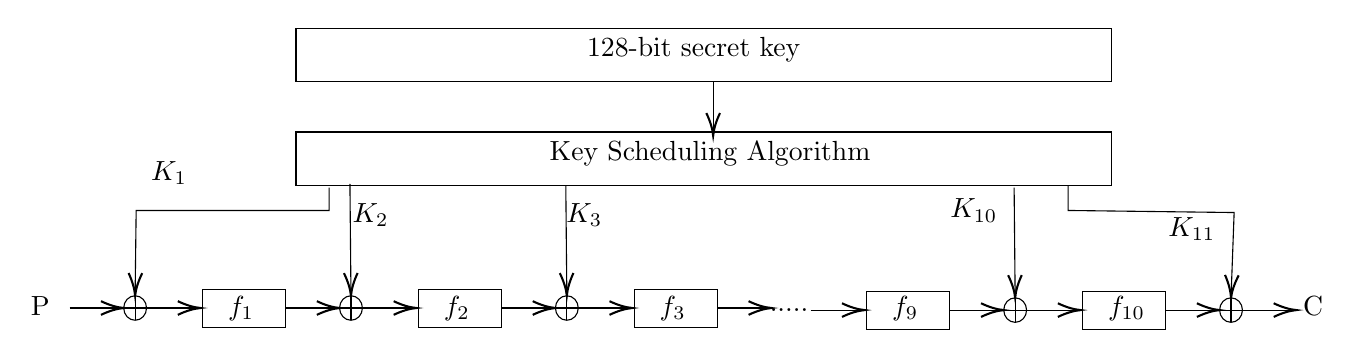
\begin{tikzpicture}[x=0.75pt,y=0.75pt,yscale=-1,xscale=1]
        \draw   (146,38) -- (539,38) -- (539,63.8) -- (146,63.8) -- cycle ;
        \draw    (347,63.8) -- (347,87.8) ;
        \draw [shift={(347,89.8)}, rotate = 270] [color={rgb, 255:red, 0; green, 0; blue, 0 }  ][line width=0.75]    (10.93,-3.29) .. controls (6.95,-1.4) and (3.31,-0.3) .. (0,0) .. controls (3.31,0.3) and (6.95,1.4) .. (10.93,3.29)   ; 
        \draw   (146,88) -- (539,88) -- (539,113.8) -- (146,113.8) -- cycle ;
        \draw    (37,172.8) -- (61,172.8) ;
        \draw [shift={(63,172.8)}, rotate = 180] [color={rgb, 255:red, 0; green, 0; blue, 0 }  ][line width=0.75]    (10.93,-3.29) .. controls (6.95,-1.4) and (3.31,-0.3) .. (0,0) .. controls (3.31,0.3) and (6.95,1.4) .. (10.93,3.29)   ;
        \draw   (63,172.8) .. controls (63,169.54) and (65.46,166.9) .. (68.5,166.9) .. controls (71.54,166.9) and (74,169.54) .. (74,172.8) .. controls (74,176.06) and (71.54,178.7) .. (68.5,178.7) .. controls (65.46,178.7) and (63,176.06) .. (63,172.8) -- cycle ; \draw   (63,172.8) -- (74,172.8) ; \draw   (68.5,166.9) -- (68.5,178.7) ;
        \draw    (74,172.8) -- (98,172.8) ;
        \draw [shift={(100,172.8)}, rotate = 180] [color={rgb, 255:red, 0; green, 0; blue, 0 }  ][line width=0.75]    (10.93,-3.29) .. controls (6.95,-1.4) and (3.31,-0.3) .. (0,0) .. controls (3.31,0.3) and (6.95,1.4) .. (10.93,3.29)   ;
        \draw   (101,163.8) -- (141,163.8) -- (141,182) -- (101,182) -- cycle ;
        \draw    (141,172.8) -- (165,172.8) ;
        \draw [shift={(167,172.8)}, rotate = 180] [color={rgb, 255:red, 0; green, 0; blue, 0 }  ][line width=0.75]    (10.93,-3.29) .. controls (6.95,-1.4) and (3.31,-0.3) .. (0,0) .. controls (3.31,0.3) and (6.95,1.4) .. (10.93,3.29)   ;
        \draw   (167,172.8) .. controls (167,169.54) and (169.46,166.9) .. (172.5,166.9) .. controls (175.54,166.9) and (178,169.54) .. (178,172.8) .. controls (178,176.06) and (175.54,178.7) .. (172.5,178.7) .. controls (169.46,178.7) and (167,176.06) .. (167,172.8) -- cycle ; \draw   (167,172.8) -- (178,172.8) ; \draw   (172.5,166.9) -- (172.5,178.7) ;
        \draw    (178,172.8) -- (202,172.8) ;
        \draw [shift={(204,172.8)}, rotate = 180] [color={rgb, 255:red, 0; green, 0; blue, 0 }  ][line width=0.75]    (10.93,-3.29) .. controls (6.95,-1.4) and (3.31,-0.3) .. (0,0) .. controls (3.31,0.3) and (6.95,1.4) .. (10.93,3.29)   ; 
        \draw   (205,163.8) -- (245,163.8) -- (245,182) -- (205,182) -- cycle ; 
        \draw    (245,172.8) -- (269,172.8) ;
        \draw [shift={(271,172.8)}, rotate = 180] [color={rgb, 255:red, 0; green, 0; blue, 0 }  ][line width=0.75]    (10.93,-3.29) .. controls (6.95,-1.4) and (3.31,-0.3) .. (0,0) .. controls (3.31,0.3) and (6.95,1.4) .. (10.93,3.29)   ; 
        \draw   (271,172.8) .. controls (271,169.54) and (273.46,166.9) .. (276.5,166.9) .. controls (279.54,166.9) and (282,169.54) .. (282,172.8) .. controls (282,176.06) and (279.54,178.7) .. (276.5,178.7) .. controls (273.46,178.7) and (271,176.06) .. (271,172.8) -- cycle ; \draw   (271,172.8) -- (282,172.8) ; \draw   (276.5,166.9) -- (276.5,178.7) ;
        \draw    (282,172.8) -- (306,172.8) ;
        \draw [shift={(308,172.8)}, rotate = 180] [color={rgb, 255:red, 0; green, 0; blue, 0 }  ][line width=0.75]    (10.93,-3.29) .. controls (6.95,-1.4) and (3.31,-0.3) .. (0,0) .. controls (3.31,0.3) and (6.95,1.4) .. (10.93,3.29)   ;
        \draw   (309,163.8) -- (349,163.8) -- (349,182) -- (309,182) -- cycle ;
        \draw    (349,172.8) -- (373,172.8) ;
        \draw [shift={(375,172.8)}, rotate = 180] [color={rgb, 255:red, 0; green, 0; blue, 0 }  ][line width=0.75]    (10.93,-3.29) .. controls (6.95,-1.4) and (3.31,-0.3) .. (0,0) .. controls (3.31,0.3) and (6.95,1.4) .. (10.93,3.29)   ;
        \draw    (394,173.8) -- (418,173.8) ;
        \draw [shift={(420,173.8)}, rotate = 180] [color={rgb, 255:red, 0; green, 0; blue, 0 }  ][line width=0.75]    (10.93,-3.29) .. controls (6.95,-1.4) and (3.31,-0.3) .. (0,0) .. controls (3.31,0.3) and (6.95,1.4) .. (10.93,3.29)   ;
        \draw   (421,164.8) -- (461,164.8) -- (461,183) -- (421,183) -- cycle ;
        \draw    (461,173.8) -- (485,173.8) ;
        \draw [shift={(487,173.8)}, rotate = 180] [color={rgb, 255:red, 0; green, 0; blue, 0 }  ][line width=0.75]    (10.93,-3.29) .. controls (6.95,-1.4) and (3.31,-0.3) .. (0,0) .. controls (3.31,0.3) and (6.95,1.4) .. (10.93,3.29)   ;
        \draw   (487,173.8) .. controls (487,170.54) and (489.46,167.9) .. (492.5,167.9) .. controls (495.54,167.9) and (498,170.54) .. (498,173.8) .. controls (498,177.06) and (495.54,179.7) .. (492.5,179.7) .. controls (489.46,179.7) and (487,177.06) .. (487,173.8) -- cycle ; \draw   (487,173.8) -- (498,173.8) ; \draw   (492.5,167.9) -- (492.5,179.7) ;
        \draw    (498,173.8) -- (522,173.8) ;
        \draw [shift={(524,173.8)}, rotate = 180] [color={rgb, 255:red, 0; green, 0; blue, 0 }  ][line width=0.75]    (10.93,-3.29) .. controls (6.95,-1.4) and (3.31,-0.3) .. (0,0) .. controls (3.31,0.3) and (6.95,1.4) .. (10.93,3.29)   ;
        \draw   (525,164.8) -- (565,164.8) -- (565,183) -- (525,183) -- cycle ;
        \draw    (565,173.8) -- (589,173.8) ;
        \draw [shift={(591,173.8)}, rotate = 180] [color={rgb, 255:red, 0; green, 0; blue, 0 }  ][line width=0.75]    (10.93,-3.29) .. controls (6.95,-1.4) and (3.31,-0.3) .. (0,0) .. controls (3.31,0.3) and (6.95,1.4) .. (10.93,3.29)   ;
        \draw   (591,173.8) .. controls (591,170.54) and (593.46,167.9) .. (596.5,167.9) .. controls (599.54,167.9) and (602,170.54) .. (602,173.8) .. controls (602,177.06) and (599.54,179.7) .. (596.5,179.7) .. controls (593.46,179.7) and (591,177.06) .. (591,173.8) -- cycle ; \draw   (591,173.8) -- (602,173.8) ; \draw   (596.5,167.9) -- (596.5,179.7) ; 
        \draw    (602,173.8) -- (626,173.8) ;
        \draw [shift={(628,173.8)}, rotate = 180] [color={rgb, 255:red, 0; green, 0; blue, 0 }  ][line width=0.75]    (10.93,-3.29) .. controls (6.95,-1.4) and (3.31,-0.3) .. (0,0) .. controls (3.31,0.3) and (6.95,1.4) .. (10.93,3.29)   ;
        \draw    (162,114.8) -- (162,125.8) -- (69,125.8) -- (68.52,164.9) ;
        \draw [shift={(68.5,166.9)}, rotate = 270.7] [color={rgb, 255:red, 0; green, 0; blue, 0 }  ][line width=0.75]    (10.93,-3.29) .. controls (6.95,-1.4) and (3.31,-0.3) .. (0,0) .. controls (3.31,0.3) and (6.95,1.4) .. (10.93,3.29)   ;
        \draw    (172,113) -- (172.48,164.9) ;
        \draw [shift={(172.5,166.9)}, rotate = 269.47] [color={rgb, 255:red, 0; green, 0; blue, 0 }  ][line width=0.75]    (10.93,-3.29) .. controls (6.95,-1.4) and (3.31,-0.3) .. (0,0) .. controls (3.31,0.3) and (6.95,1.4) .. (10.93,3.29)   ;
        \draw    (276,113.8) -- (276.48,164.9) ;
        \draw [shift={(276.5,166.9)}, rotate = 269.46] [color={rgb, 255:red, 0; green, 0; blue, 0 }  ][line width=0.75]    (10.93,-3.29) .. controls (6.95,-1.4) and (3.31,-0.3) .. (0,0) .. controls (3.31,0.3) and (6.95,1.4) .. (10.93,3.29)   ;
        \draw    (492,114.8) -- (492.48,165.9) ;
        \draw [shift={(492.5,167.9)}, rotate = 269.46] [color={rgb, 255:red, 0; green, 0; blue, 0 }  ][line width=0.75]    (10.93,-3.29) .. controls (6.95,-1.4) and (3.31,-0.3) .. (0,0) .. controls (3.31,0.3) and (6.95,1.4) .. (10.93,3.29)   ;
        \draw    (518,113.8) -- (518,125.8) -- (598,126.8) -- (596.57,165.9) ;
        \draw [shift={(596.5,167.9)}, rotate = 272.09] [color={rgb, 255:red, 0; green, 0; blue, 0 }  ][line width=0.75]    (10.93,-3.29) .. controls (6.95,-1.4) and (3.31,-0.3) .. (0,0) .. controls (3.31,0.3) and (6.95,1.4) .. (10.93,3.29)   ;
        
        \draw (285,41) node [anchor=north west][inner sep=0.75pt]   [align=left] {128-bit secret key};
        \draw (267,91) node [anchor=north west][inner sep=0.75pt]   [align=left] {Key Scheduling Algorithm};
        \draw (17,166) node [anchor=north west][inner sep=0.75pt]   [align=left] {P};
        \draw (112,166) node [anchor=north west][inner sep=0.75pt]   [align=left] {$f_1$};
        \draw (216,166) node [anchor=north west][inner sep=0.75pt]   [align=left] {$f_2$};
        \draw (320,166) node [anchor=north west][inner sep=0.75pt]   [align=left] {$f_3$};
        \draw (373,172) node [anchor=north west][inner sep=0.75pt]   [align=left] {.....};
        \draw (432,166) node [anchor=north west][inner sep=0.75pt]   [align=left] {$f_9$};
        \draw (536,166) node [anchor=north west][inner sep=0.75pt]   [align=left] {$f_{10}$};
        \draw (630,166) node [anchor=north west][inner sep=0.75pt]   [align=left] {C};
        \draw (75,101) node [anchor=north west][inner sep=0.75pt]   [align=left] {$K_1$};
        \draw (172,121) node [anchor=north west][inner sep=0.75pt]   [align=left] {$K_2$};
        \draw (275,121) node [anchor=north west][inner sep=0.75pt]   [align=left] {$K_3$};
        \draw (460,119) node [anchor=north west][inner sep=0.75pt]   [align=left] {$K_{10}$};
        \draw (565,128) node [anchor=north west][inner sep=0.75pt]   [align=left] {$K_{11}$};
    \end{tikzpicture}
    \caption{AES Structure}
\end{center}

\section{Components of AES}

\subsection{Round Function of AES}
The Advanced Encryption Standard (AES) employs a round function to iteratively transform plaintext blocks into ciphertext blocks. This round function, denoted as \( f \), comprises various operations applied sequentially, including substitution, permutation, and mixing. Each round function \( f_i \), where \( i \) ranges from 1 to 10, maps from a 128-bit input to a 128-bit output:

\[ f_i : \{0, 1\}^{128} \rightarrow \{0, 1\}^{128} \quad \text{for} \quad 1 \leq i \leq 10 \]\\
The Subbytes operation is a bijective mapping from 128 bits to 128 bits:

\[ \text{Subbytes} : \{0, 1\}^{128} \rightarrow \{0, 1\}^{128} \]

\subsubsection{Substitution (SubBytes)}

The SubBytes step of AES replaces each byte in the state matrix with another byte using a substitution table called the S-box. This table performs a non-linear byte substitution, which helps enhance the confusion property of AES.\\\\
For a byte at row \(i\) and column \(j\) of the state matrix \(S\), denoted as \(S_{i,j}\), the substitution is calculated as:

\[ \text{SubBytes}(S)_{i,j} = \text{S-box}(S_{i,j}) \]\\
The input \(S\) to the SubBytes function is a 128-bit binary input. A \(4 \times 4\) matrix can be constructed from this input by arranging the bits in a specific manner.

\begin{center}
    $S \rightarrow  
        \begin{bmatrix}
        S_{00} & S_{01} & S_{02} & S_{03}\\
        S_{10} & S_{11} & S_{12} & S_{13}\\
        S_{20} & S_{21} & S_{22} & S_{23}\\
        S_{30} & S_{31} & S_{32} & S_{33}\\
        \end{bmatrix}$
\end{center}
\\where $S_{ij}$ is a byte (8-bits). Consider the 128-bit plaintext of 128-bit. The plaintext again can be written as a $4 \times 4$ matrix in the following way. Keep in mind, the ordering of the plaintext bytes.\\
\begin{center}
    $P = P_0P_1P_2....P_{15}$, length of each $P_i$ is 8-bit\\
    \vspace{5mm}
    $P \rightarrow  
        \begin{bmatrix}
        P_0 & P_4 & P_8 & P_{12}\\
        P_1 & P_5 & P_9 & P_{13}\\
        P_2 & P_6 & P_{10} & P_{14}\\
        P_3 & P_7 & P_{11} & P_{15}\\
        \end{bmatrix}$
\end{center}
Similarly, the first round key $K_1$ can also be written as a matrix.
\begin{center}
    $K_1 = K_0K_1K_2....K_{15}$, length of each $K_i$ is 8-bit\\\\
    \vspace{5mm}
    $K_1 \rightarrow  
        \begin{bmatrix}
        K_0 & K_4 & K_8 & K_{12}\\
        K_1 & K_5 & K_9 & K_{13}\\
        K_2 & K_6 & K_{10} & K_{14}\\
        K_3 & K_7 & K_{11} & K_{15}\\
        \end{bmatrix}$
\end{center}
For AES-128, we first xor the plaintext with the first round key $K_1$. The output is then passed to first round function, wherein, it is first passed to subbytes function.
\begin{center}
    $S = (S_{ij})_{4 \times 4} = P \oplus K_1$
\end{center}
The output after the subbyte function is performed on S is $S'$.
\begin{center}
    $S' = Subbytes(S)$
\end{center}

\noindent
\begin{figure}[H]
    \centering
    \fbox{\begin{minipage}{0.9\textwidth}
    We will see an overview of the subbyte function. Below are the steps involved:
    \begin{enumerate}
        \item A constant C = $C_7C_6C_5C_4C_3C_2C_1C_0 = (01100011) = (63)_{16}$ is declared.
        \item Substitution box $\mathbb{S}$ maps every element of the S matrix from 8-bit to 8-bit. This $\mathbb{S}$ box is applied to every element of S matrix, i.e., $S_{ij}$. Therefore, it is an 8-bit to 8-bit mapping. Also, $\mathbb{S}(0) = 0$ is taken as a rule (fixed for AES).
        \item Suppose $\mathbb{S}(S_{ij}) = m_7m_6m_5m_4m_3m_2m_1m_0$.
        \item For $i = 0$ to $i = 7$, compute $b_i$ as:
        \[
        b_i = (m_i + m_{(i+4)\%8} + m_{(i+5)\%8} + m_{(i+6)\%8} + m_{(i+7)\%8} + C_i) \% 2
        \]
        \item Therefore, the output is $b_7b_6b_5b_4b_3b_2b_1b_0$.
        \item $S'_{ij} = (b_7b_6b_5b_4b_3b_2b_1b_0)$
    \end{enumerate}
   
    \end{minipage}}
    \label{fig:your_label}
\end{figure}
\noindent
Hence, $S'_{ij}$ is computed for each $S_{ij}$, and the output matrix is the output of the subbyte function.
    \[
    \begin{bmatrix}
        S_{00} & S_{01} & S_{02} & S_{03}\\
        S_{10} & S_{11} & S_{12} & S_{13}\\
        S_{20} & S_{21} & S_{22} & S_{23}\\
        S_{30} & S_{31} & S_{32} & S_{33}\\
    \end{bmatrix}
    \xrightarrow{Subbyte}
    \begin{bmatrix}
        S'_{00} & S'_{01} & S'_{02} & S'_{03}\\
        S'_{10} & S'_{11} & S'_{12} & S'_{13}\\
        S'_{20} & S'_{21} & S'_{22} & S'_{23}\\
        S'_{30} & S'_{31} & S'_{32} & S'_{33}\\
    \end{bmatrix}
    \]
\noindent
Now, we will discuss the substitution box $\mathbb{S}$ that takes 8-bit input and produces 8-bit output.
\begin{center}
    $\mathbb{S}: \{0, 1\}^8 \rightarrow \{0, 1\}^8$ and $\mathbb{S}(0) = 0$
\end{center}
Let's say input X is given to this $\mathbb{S}$ box and $X \neq 0$. We need to find $Y = \mathbb{S}(X)$.
\begin{center}
    $X = a_7a_6a_5a_4a_3a_2a_1a_0$, where $a_i \in \{0, 1\}$
\end{center}
We can construct a polynomial $P(x)$ using the bits of X as coefficients.
\begin{center}
    $P(x) = a_0 + a_1 \cdot x + a_2 \cdot x^2 +.....+ a_7 \cdot x^7$
\end{center}
\vspace{3mm}
Clearly, degree of $P(x) \leq 7$. Also, $P(x) \in F_2[x]$. Moreover, since $X \neq 0 \implies P(x) \neq 0$. Another polynomial $g(x) = x^8 + x^4 + x^3 + x + 1$ is fixed for AES. $g(x)$ is a primitive polynomial.\\
\newline
Given that $g(x)$ is a primitive polynomial, it defines a field denoted by $(\mathbb{F}_2[x]/\langle g(x) \rangle, +, *)$, where $+$ and $*$ represent addition and multiplication modulo $g(x)$, respectively. All polynomials within this field have a maximum degree of $7$. Consequently, $P(x)$ is a member of this field. Moreover, since $\langle g(x) \rangle$ is primitive, we can ascertain the multiplicative inverse of any polynomial in $(\mathbb{F}_2[x]/\langle g(x) \rangle)$. Hence, we aim to determine the multiplicative inverse of $P(x)$ modulo $g(x)$, denoted as $q(x)$.

\begin{center}
    $P(x)\cdot q(x) \equiv 1 mod $ $g(x)$\\
    \vspace{1mm}
    $P(x) \cdot q(x) \equiv 1 mod (x^8 + x^4 + x^3 + x + 1)$\\
    \vspace{1mm}
    $P(x)\cdot q(x) - 1 = h(x) \cdot (x^8 + x^4 + x^3 + x + 1)$\\
    \vspace{1mm}
    $1 = P(x) \cdot q(x) + h(x) \cdot (x^8 + x^4 + x^3 + x + 1)$
\end{center}
Therefore, we can find the $q(x)$ with the help of Extended Euclidean Algorithm. Also, $q(x)$ will be a polynomial of degree at most 7.
\begin{center}
    $q(x) = r_0 + r_1\cdot x+ r_2 \cdot x^2 +.....+ r_7 \cdot x^7$, where $r_i \in \{0, 1\}$
\end{center}
From the coefficients, we can build a 8-bit binary string as $r_7r_6r_5r_4r_3r_2r_1r_0$. This string is the output of the $\mathbb{S}$ box. Therefore,
\begin{center}
    $\mathbb{S}(X) = Y = (r_7r_6r_5r_4r_3r_2r_1r_0)$
\end{center}

\noindent
\textbf{Example:} Find Subbytes(01010011).\\\\
\textbf{Solution:} X = 01010011, therefore $P(x) = x^6 + x^4 + x + 1$. Also, $g(x) = x^8 + x^4 + x^3 + x + 1$. Now, let's perform the Extended Euclidean Algorithm.
\begin{center}
    \tikzset{every picture/.style={line width=0.75pt}} 

    \begin{tikzpicture}[x=0.75pt,y=0.75pt,yscale=-1,xscale=1]
%uncomment if require: \path (0,529); %set diagram left start at 0, and has height of 529
        
        %Straight Lines [id:da7065959490003173] 
        \draw    (163,171.2) -- (363,171.2) ;
        %Straight Lines [id:da028549667874976592] 
        \draw    (182,230.2) -- (339,231.2) ;
        %Straight Lines [id:da899367259935002] 
        \draw    (186,283.2) -- (343,284.2) ;
        %Straight Lines [id:da4356732499452918] 
        \draw    (292,284.2) -- (449,285.2) ;
        %Straight Lines [id:da9322638753565391] 
        \draw    (304,336.2) -- (439,337.2) ;
        %Straight Lines [id:da9488931091504231] 
        \draw    (359,381.2) -- (510,381.2) ;
        %Straight Lines [id:da18220626076094226] 
        \draw    (446,441.2) -- (510,440.2) ;
        %Straight Lines [id:da7371705002655333] 
        \draw    (488,481.2) -- (528,480.2) ;
        %Straight Lines [id:da7407976464457187] 
        \draw    (489,501.2) -- (529,500.2) ;
        
        \draw (158,169) node [anchor=north west][inner sep=0.75pt]   [align=left] {{\Huge )}};
        \draw (187,178) node [anchor=north west][inner sep=0.75pt]   [align=left] {$x^8 + x^4 + x^3 + x + 1$};
        \draw (351,169) node [anchor=north west][inner sep=0.75pt]   [align=left] {{\Huge (}};
        \draw (60,177) node [anchor=north west][inner sep=0.75pt]   [align=left] {$x^6 + x^4 + x + 1$};
        \draw (359,177) node [anchor=north west][inner sep=0.75pt]   [align=left] {$x^2 + 1$};
        \draw (185,205) node [anchor=north west][inner sep=0.75pt]   [align=left] {$x^8 + x^6 + x^3 + x^2$};
        \draw (186,238) node [anchor=north west][inner sep=0.75pt]   [align=left] {$x^6 + x^4 + x^2 + x + 1$};
        \draw (185,261) node [anchor=north west][inner sep=0.75pt]   [align=left] {$x^6 + x^4 + x + 1$};
        \draw (285,282) node [anchor=north west][inner sep=0.75pt]   [align=left] {{\Huge )}};
        \draw (438,283) node [anchor=north west][inner sep=0.75pt]   [align=left] {{\Huge (}};
        \draw (267,290) node [anchor=north west][inner sep=0.75pt]   [align=left] {$x^2$};
        \draw (453,292) node [anchor=north west][inner sep=0.75pt]   [align=left] {$x^4 + x^2$};
        \draw (314,289) node [anchor=north west][inner sep=0.75pt]   [align=left] {$x^6 + x^4 + x + 1$};
        \draw (315,315) node [anchor=north west][inner sep=0.75pt]   [align=left] {$x^6$};
        \draw (358,338) node [anchor=north west][inner sep=0.75pt]   [align=left] {$x^4+ x + 1$};
        \draw (359,359) node [anchor=north west][inner sep=0.75pt]   [align=left] {$x^4$};
        \draw (399,387) node [anchor=north west][inner sep=0.75pt]   [align=left] {$x + 1$};
        \draw (433,379) node [anchor=north west][inner sep=0.75pt]   [align=left] {{\Huge )}};
        \draw (497,380) node [anchor=north west][inner sep=0.75pt]   [align=left] {{\Huge (}};
        \draw (460,387) node [anchor=north west][inner sep=0.75pt]   [align=left] {$x^2$};
        \draw (515,386) node [anchor=north west][inner sep=0.75pt]   [align=left] {$x + 1$};
        \draw (448,416) node [anchor=north west][inner sep=0.75pt]   [align=left] {$x^2 + x$};
        \draw (486,445) node [anchor=north west][inner sep=0.75pt]   [align=left] {$x$};
        \draw (486,458) node [anchor=north west][inner sep=0.75pt]   [align=left] {$x + 1$};
        \draw (508,482.7) node [anchor=north west][inner sep=0.75pt]   [align=left] {$1$};
    \end{tikzpicture}
\end{center}

Now, let's work upside down to find the multiplicative inverse. Therefore,
    $1 = q(x)\cdot P(x) = h(x) \cdot g(x)$\\\\
    \vspace{2mm}
    $1 = 1 \cdot x^2 + (x+1) \cdot (x+1)$\\
    \vspace{2mm}
    $1 = x^2 + (x + 1) \cdot [(x^6 + x^4 + x + 1) + x^2 \cdot (x^4 + x^2)]$\\
    \vspace{2mm}
    $1 = (x+1) \cdot (x^6 + x^4 + x + 1) + x^2 \cdot [1 + (x+1) \cdot (x^4 + x^2)]$\\
    \vspace{2mm}
    $1 = (x+1) \cdot (x^6 + x^4 + x + 1) + x^2 \cdot (x^5 + x^4 + x^3 + x^2 + 1)$\\
    \vspace{2mm}
    $1 = (x+1) \cdot (x^6 + x^4 + x + 1) + (x^5 + x^4 + x^3 + x^2 + 1) \cdot [(x^8 + x^4 + x^3 + x + 1) + (x^6 + x^4 + x + 1) \cdot (x^2 + 1)] $\\
    \vspace{2mm}
    $1 = [(x + 1) + (x^2 + 1) \cdot (x^5 + x^4 + x^3 + x^2 + 1)] \cdot P(x) + (x^5 + x^4 + x^3 + x^2 + 1) \cdot g(x)$\\
    \vspace{2mm}
    $1 = (x + 1 + x^7 + x^6 + x^5 + x^4 + x^2 + x^5 + x^4 + x^3 + x^2 + 1) \cdot P(x) + (x^5 + x^4 + x^3 + x^2 + 1) \cdot g(x)$\\
    \vspace{2mm}
    $1 = (x^7 + x^6 + x^3 + x) \cdot P(x) + (x^5 + x^4 + x^3 + x^2 + 1) \cdot g(x)$\\\\
Therefore, Multiplicative Inverse of P(x) is $q(x) = x^7 + x^6 + x^3 + x$. Therefore,
\begin{center}
    $\mathbb{S}(01010011) = (11001010) = m_7m_6m_5m_4m_3m_2m_1m_0$
\end{center}
\vspace{2mm}
Now, let's compute $b_7b_6b_5b_4b_3b_2b_1b_0$. The constant C = $c_7c_6c_5c_4c_3c_2c_1c_0 = 01100011$.
\begin{center}
    \begin{tabular}{|c|c|c|c|c|c|c|c|c|}
        \hline
         & 0 & 1 & 2 & 3 & 4 & 5 & 6 & 7 \\ \hline
        c & 1 & 1 & 0 & 0 & 0 & 1 & 1 & 0  \\ \hline
        m & 0 & 1 & 0 & 1 & 0 & 0 & 1 & 1  \\ \hline
    \end{tabular}
\end{center}
\begin{center}
    $b_0 = (0 + 0 + 0 + 1 + 1 + 1) \% 2 = 1$\\
    $b_1 = (1 + 0 + 1 + 1 + 0 + 1) \%2 = 0$\\
    $b_2 = 1, b_3 = 1, b_4 = 0$\\
    $b_5 = 1, b_6 = 1, b_7 = 1$\\
    $\therefore subbytes(01010011) = b_7b_6b_5b_4b_3b_2b_1b_0 = (11101101)$\\
    $subbytes(53) = (ED)$
\end{center}

\noindent
The value returned by the $subbyte$ function is a hexadecimal number. The first four digits give the row number, the next four digits give the column numbers, and together they highlight the cell in a 16x16 table, which contains the required encrypted characters.
\begin{center}
    Input = XY\\
    \vspace{2mm}
    Subbyte(Input) $\rightarrow$ element present in row number X and column number Y
\end{center}
\vspace{2mm}
The lookup table is given in the diagram below - 

\[
\begin{array}{|c|c|c|c|c|c|c|c|c|c|c|c|c|c|c|c|c|}
\hline
\text{Input} & 00 & 01 & 02 & 03 & 04 & 05 & 06 & 07 & 08 & 09 & 0A & 0B & 0C & 0D & 0E & 0F \\
\hline
00 & 63 & 7C & 77 & 7B & F2 & 6B & 6F & C5 & 30 & 01 & 67 & 2B & FE & D7 & AB & 76 \\
01 & CA & 82 & C9 & 7D & FA & 59 & 47 & F0 & AD & D4 & A2 & AF & 9C & A4 & 72 & C0 \\
02 & B7 & FD & 93 & 26 & 36 & 3F & F7 & CC & 34 & A5 & E5 & F1 & 71 & D8 & 31 & 15 \\
03 & 04 & C7 & 23 & C3 & 18 & 96 & 05 & 9A & 07 & 12 & 80 & E2 & EB & 27 & B2 & 75 \\
04 & 09 & 83 & 2C & 1A & 1B & 6E & 5A & A0 & 52 & 3B & D6 & B3 & 29 & E3 & 2F & 84 \\
05 & 53 & D1 & 00 & ED & 20 & FC & B1 & 5B & 6A & CB & BE & 39 & 4A & 4C & 58 & CF \\
06 & D0 & EF & AA & FB & 43 & 4D & 33 & 85 & 45 & F9 & 02 & 7F & 50 & 3C & 9F & A8 \\
07 & 51 & A3 & 40 & 8F & 92 & 9D & 38 & F5 & BC & B6 & DA & 21 & 10 & FF & F3 & D2 \\
08 & CD & 0C & 13 & EC & 5F & 97 & 44 & 17 & C4 & A7 & 7E & 3D & 64 & 5D & 19 & 73 \\
09 & 60 & 81 & 4F & DC & 22 & 2A & 90 & 88 & 46 & EE & B8 & 14 & DE & 5E & 0B & DB \\
0A & E0 & 32 & 3A & 0A & 49 & 06 & 24 & 5C & C2 & D3 & AC & 62 & 91 & 95 & E4 & 79 \\
0B & E7 & C8 & 37 & 6D & 8D & D5 & 4E & A9 & 6C & 56 & F4 & EA & 65 & 7A & AE & 08 \\
0C & BA & 78 & 25 & 2E & 1C & A6 & B4 & C6 & E8 & DD & 74 & 1F & 4B & BD & 8B & 8A \\
0D & 70 & 3E & B5 & 66 & 48 & 03 & F6 & 0E & 61 & 35 & 57 & B9 & 86 & C1 & 1D & 9E \\
0E & E1 & F8 & 98 & 11 & 69 & D9 & 8E & 94 & 9B & 1E & 87 & E9 & CE & 55 & 28 & DF \\
0F & 8C & A1 & 89 & 0D & BF & E6 & 42 & 68 & 41 & 99 & 2D & 0F & B0 & 54 & BB & 16 \\
\hline
\end{array}
\]


\subsubsection{Permutation (ShiftRows)}

In the ShiftRows step, bytes in each row of the state matrix are cyclically shifted to the left. This permutation operation provides diffusion, spreading the influence of each byte throughout the state matrix.

\[
\text{{ShiftRows}}(S) = 
\begin{pmatrix}
S_{0,0} & S_{0,1} & S_{0,2} & S_{0,3} \\
S_{1,1} & S_{1,2} & S_{1,3} & S_{1,0} \\
S_{2,2} & S_{2,3} & S_{2,0} & S_{2,1} \\
S_{3,3} & S_{3,0} & S_{3,1} & S_{3,2} \\
\end{pmatrix}
\]\\
Shift Row function is a mapping from 128-bit to 128-bit. It takes a $4 \times 4$ matrix as input (the output of Subbyte function). It performs left circular shift on the elements of $i^{th}$ row by $i$ positions, where row index begins from 0.
\begin{center}
    Shift Rows: $\{0, 1\}^{128} \rightarrow \{0, 1\}^{128}$\\
    \vspace{5mm}
    $
    \begin{bmatrix}
        S_{00} & S_{01} & S_{02} & S_{03}\\
        S_{10} & S_{11} & S_{12} & S_{13}\\
        S_{20} & S_{21} & S_{22} & S_{23}\\
        S_{30} & S_{31} & S_{32} & S_{33}\\
    \end{bmatrix}
    \xrightarrow{Shift Rows}
    \begin{bmatrix}
        S_{00} & S_{01} & S_{02} & S_{03}\\
        S_{11} & S_{12} & S_{13} & S_{10}\\
        S_{22} & S_{23} & S_{20} & S_{21}\\
        S_{33} & S_{30} & S_{31} & S_{32}\\
    \end{bmatrix}
    $
\end{center}

\subsubsection{Mixing (MixColumns)}

MixColumns is a linear transformation that operates on each column of the state matrix independently. It involves multiplying each column by a fixed matrix and then applying modular polynomial arithmetic. This mixing operation increases the diffusion further.

\[
\text{{MixColumns}}(S) = 
\begin{pmatrix}
2 & 3 & 1 & 1 \\
1 & 2 & 3 & 1 \\
1 & 1 & 2 & 3 \\
3 & 1 & 1 & 2 \\
\end{pmatrix} \times
\begin{pmatrix}
S_{0,0} & S_{0,1} & S_{0,2} & S_{0,3} \\
S_{1,0} & S_{1,1} & S_{1,2} & S_{1,3} \\
S_{2,0} & S_{2,1} & S_{2,2} & S_{2,3} \\
S_{3,0} & S_{3,1} & S_{3,2} & S_{3,3} \\
\end{pmatrix}
\]\\
Mix columns, again, is a mapping from 128-bit to 128-bit. It also takes a $4 \times 4$ matrix as input (the output of Shift Rows function).
\begin{center}
    Mix Columns: $\{0, 1\}^{128} \rightarrow \{0, 1\}^{128}$\\
    \vspace{5mm}
    $(S_{ij})_{4 \times 4} \xrightarrow{Mix Columns} (S_{ij}^{'})_{4 \times 4}$
\end{center}
\vspace{2mm}
Consider the column $c \in {0,1,2,3}$ of matrix S.
\begin{center}
    column = $\begin{bmatrix}
        S_{0c}\\
        S_{1c}\\
        S_{2c}\\
        S_{3c}\\
    \end{bmatrix}$
\end{center}
\vspace{2mm}
The Mix Columns function is defined as follows. For i = 0 to i = 3, let $t_i$ be the polynomial constructed from $S_{ic}$. Define four polynomials as:
\begin{center}
    $u_0 = [(x * t_0) + (x + 1) * t_1 + t_2 + t_3]$ mod $(x^8 + x^4 + x^3 + x + 1)$\\
    \vspace{1mm}
    $u_1 = [t_0 + (x * t_1) + (x + 1) * t_2 + t_3]$ mod $(x^8 + x^4 + x^3 + x + 1)$\\
    \vspace{1mm}
    $u_2 = [t_0 + t_1 + (x * t_2) + (x + 1) * t_3]$ mod $(x^8 + x^4 + x^3 + x + 1)$\\
    \vspace{1mm}
    $u_3 = [(x + 1) * t_0 + t_1 + t_2 + (x * t_3)]$ mod $(x^8 + x^4 + x^3 + x + 1)$\\
\end{center}
Now, $S_{ij}^{'}$ is the binary 8-bits constructed using $u_i$. Therefore, 
\begin{center}
    $\begin{bmatrix}
        S_{0c}\\
        S_{1c}\\
        S_{2c}\\
        S_{3c}\\
    \end{bmatrix}
    \xrightarrow{Mix Columns}
    \begin{bmatrix}
        S_{0c}^{'}\\
        S_{1c}^{'}\\
        S_{2c}^{'}\\
        S_{3c}^{'}\\
    \end{bmatrix}$
\end{center}
Applying Mix Columns to each columns, will give us the entire $(S_{ij}^{'})_{4 \times 4}$ matrix. Therefore, Mix Column can be defined as a matrix multiplication as:
\begin{center}
    $
    (S_{ij}^{'})_{4 \times 4} = 
    \begin{bmatrix}
        x & x + 1 & 1 & 1\\
        1 & x & x+1 & 1\\
        1 & 1 & x & x+1\\
        x+1 & 1 & 1 & x\\
    \end{bmatrix}
    \times
    \begin{bmatrix}
        S_{00} & S_{01} & S_{02} & S_{03}\\
        S_{10} & S_{11} & S_{12} & S_{13}\\
        S_{20} & S_{21} & S_{22} & S_{23}\\
        S_{30} & S_{31} & S_{32} & S_{33}\\\\
    \end{bmatrix}
    $
    mod $(x^8 + x^4 + x^3 + x + 1)$
\end{center}

\noindent
The polynomial $(x^8 + x^4 + x^3 + x + 1)$ is a primitive polynomial, hence, it is possible to construct the inverse of the Mix Columns function.

\subsubsection{Combining everything together!}

The round function $F$ is a composition of these three operations:
\[
f(S) = \text{{MixColumns}}(\text{{ShiftRows}}(\text{{SubBytes}}(S)))
\]
\noindent
For the first 9 round functions:
\begin{center}
    $f_i(X) = MixColumns(ShiftRows(Subbytes(X)))$ $\forall$ $1 \leq i \leq 9$
\end{center}

\noindent
However, the last round function $f_{10}$ is based on subbytes and shift rows only. Therefore,
\begin{center}
    $f_{10}(X) = ShiftRows(Subbytes(X))$
\end{center}

\noindent
Each Subbyte, Shift Rows and Mix Columns is a bijection from 128-bit to 128-bit. This means each of them has existing inverse. Therefore, given $y = f_i(X)$, to get $X$, apply inverse of mix columns, then apply inverse of Shift Rows and then apply inverse of Subbytes.\\

\noindent
For the first 9 rounds $f_1, f_2,..., f_9$:\\
\begin{center}
    \tikzset{every picture/.style={line width=0.75pt}} 
    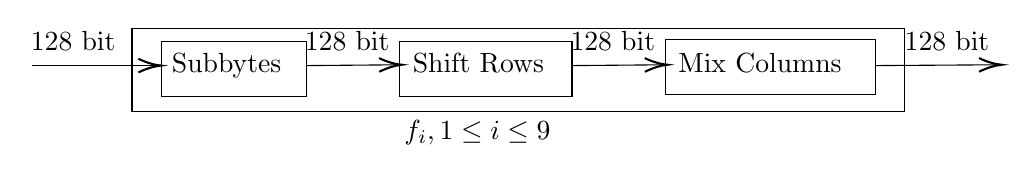
\begin{tikzpicture}[x=0.75pt,y=0.75pt,yscale=-1,xscale=1]
        \draw   (139,298.6) -- (511,298.6) -- (511,338.6) -- (139,338.6) -- cycle ;
        \draw   (153,305.2) -- (223,305.2) -- (223,331.6) -- (153,331.6) -- cycle ;
        \draw   (268,305.2) -- (351,305.2) -- (351,331.6) -- (268,331.6) -- cycle ;
        \draw   (396,304.2) -- (497,304.2) -- (497,330.6) -- (396,330.6) -- cycle ;
        \draw    (223,316.6) -- (267,316.22) ;
        \draw [shift={(269,316.2)}, rotate = 179.5] [color={rgb, 255:red, 0; green, 0; blue, 0 }  ][line width=0.75]    (10.93,-3.29) .. controls (6.95,-1.4) and (3.31,-0.3) .. (0,0) .. controls (3.31,0.3) and (6.95,1.4) .. (10.93,3.29)   ;
        \draw    (351,316.6) -- (395,316.22) ;
        \draw [shift={(397,316.2)}, rotate = 179.5] [color={rgb, 255:red, 0; green, 0; blue, 0 }  ][line width=0.75]    (10.93,-3.29) .. controls (6.95,-1.4) and (3.31,-0.3) .. (0,0) .. controls (3.31,0.3) and (6.95,1.4) .. (10.93,3.29)   ;
        \draw    (91,316.6) -- (151,316.6) ;
        \draw [shift={(153,316.6)}, rotate = 180] [color={rgb, 255:red, 0; green, 0; blue, 0 }  ][line width=0.75]    (10.93,-3.29) .. controls (6.95,-1.4) and (3.31,-0.3) .. (0,0) .. controls (3.31,0.3) and (6.95,1.4) .. (10.93,3.29)   ;
        \draw    (497,316.6) -- (556,316.21) ;
        \draw [shift={(558,316.2)}, rotate = 179.62] [color={rgb, 255:red, 0; green, 0; blue, 0 }  ][line width=0.75]    (10.93,-3.29) .. controls (6.95,-1.4) and (3.31,-0.3) .. (0,0) .. controls (3.31,0.3) and (6.95,1.4) .. (10.93,3.29)   ;
        
        \draw (157,309.2) node [anchor=north west][inner sep=0.75pt]   [align=left] {Subbytes};
        \draw (273,309.2) node [anchor=north west][inner sep=0.75pt]   [align=left] {Shift Rows};
        \draw (401,309.2) node [anchor=north west][inner sep=0.75pt]   [align=left] {Mix Columns};
        \draw (221,298.6) node [anchor=north west][inner sep=0.75pt]   [align=left] {128 bit};
        \draw (349,298.6) node [anchor=north west][inner sep=0.75pt]   [align=left] {128 bit};
        \draw (89,298.6) node [anchor=north west][inner sep=0.75pt]   [align=left] {128 bit};
        \draw (510,298.6) node [anchor=north west][inner sep=0.75pt]   [align=left] {128 bit};
        \draw (269,341.6) node [anchor=north west][inner sep=0.75pt]   [align=left] {$f_i, 1 \leq i \leq 9$};
    \end{tikzpicture}
\end{center}

\noindent
For the last round function $f_{10}$:\\
\begin{center}
    \tikzset{every picture/.style={line width=0.75pt}} 

    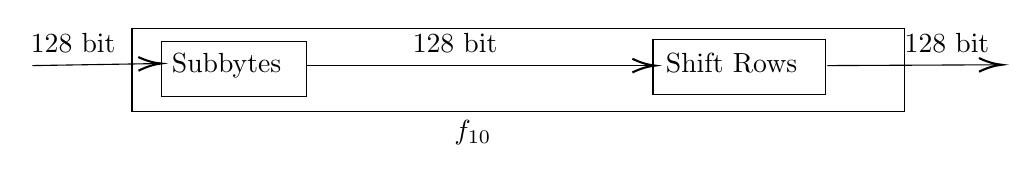
\begin{tikzpicture}[x=0.75pt,y=0.75pt,yscale=-1,xscale=1] 
        \draw   (146,426.6) -- (518,426.6) -- (518,466.6) -- (146,466.6) -- cycle ;
        \draw   (160,433.2) -- (230,433.2) -- (230,459.6) -- (160,459.6) -- cycle ;
        \draw   (397,432.2) -- (480,432.2) -- (480,458.6) -- (397,458.6) -- cycle ;
        \draw    (230,444.6) -- (396,444.6) ;
        \draw [shift={(398,444.6)}, rotate = 180] [color={rgb, 255:red, 0; green, 0; blue, 0 }  ][line width=0.75]    (10.93,-3.29) .. controls (6.95,-1.4) and (3.31,-0.3) .. (0,0) .. controls (3.31,0.3) and (6.95,1.4) .. (10.93,3.29)   ; 
        \draw    (98,444.6) -- (158,443.63) ;
        \draw [shift={(160,443.6)}, rotate = 179.08] [color={rgb, 255:red, 0; green, 0; blue, 0 }  ][line width=0.75]    (10.93,-3.29) .. controls (6.95,-1.4) and (3.31,-0.3) .. (0,0) .. controls (3.31,0.3) and (6.95,1.4) .. (10.93,3.29)   ;
        \draw    (481,444.6) -- (563,444.21) ;
        \draw [shift={(565,444.2)}, rotate = 179.73] [color={rgb, 255:red, 0; green, 0; blue, 0 }  ][line width=0.75]    (10.93,-3.29) .. controls (6.95,-1.4) and (3.31,-0.3) .. (0,0) .. controls (3.31,0.3) and (6.95,1.4) .. (10.93,3.29)   ;
        
        \draw (164,437.2) node [anchor=north west][inner sep=0.75pt]   [align=left] {Subbytes};
        \draw (402,437.2) node [anchor=north west][inner sep=0.75pt]   [align=left] {Shift Rows};
        \draw (280,427.6) node [anchor=north west][inner sep=0.75pt]   [align=left] {128 bit};
        \draw (96,427.6) node [anchor=north west][inner sep=0.75pt]   [align=left] {128 bit};
        \draw (517,427.6) node [anchor=north west][inner sep=0.75pt]   [align=left] {128 bit};
        \draw (300,469.6) node [anchor=north west][inner sep=0.75pt]   [align=left] {$f_{10}$};
    \end{tikzpicture}
\end{center}


\subsection{Key Scheduling Algorithm of AES-128}

The AES-128 key scheduling algorithm operates on a 128-bit encryption key, producing 11 distinct round keys, each consisting of 128 bits. The key is represented as \( (key[0], key[1], ..., key[15]) \), where each \( key[i] \) is a single byte. This process involves generating 44 words, each 32 bits long, denoted as \( w[0], w[1], ..., w[43] \). Notably, \( \frac{{32 \times 44}}{128} = 11 \), providing the necessary material for creating 11 round keys from these 44 words.\\\\
The AES-128 key scheduling algorithm comprises two essential functions:

\begin{enumerate}
    \item \textbf{ROTWORD(\(B_0B_1B_2B_3\)):} This function takes a word as input and performs a left circular shift of its constituent bytes, equivalent to a rotation by 8 bits. The input word, represented by \( B_0, B_1, B_2, B_3 \), undergoes transformation, resulting in the output: \( \text{ROTWORD}(B_0B_1B_2B_3) = B_1B_2B_3B_0 \).
    
    \item \textbf{SUBWORD(\(B_0B_1B_2B_3\)):} This function operates on a word, initiating the Subbyte operation, which is crucial to the round function of AES, on each of its constituent bytes \( B_0, B_1, B_2, B_3 \). Consequently, the output of the SUBWORD function takes the form:\\ \( \text{SUBWORD}(B_0B_1B_2B_3) = B'_0B'_1B'_2B'_3 \), where \( B'_i = \text{Subbytes}(B_i) \) for all \( i \in \{0, 1, 2, 3\} \).
\end{enumerate}\\
\vspace{3mm}
In the AES-128 key scheduling algorithm, ten round constants are employed, each represented as a 32-bit word in hexadecimal format.\\\\
In the AES-128 key scheduling algorithm, ten round constants are utilized, each represented as a 32-bit word in hexadecimal format:

\begin{center}
    $RCON[1] = 0x01000000$\\
    $RCON[2] = 0x02000000$\\
    $RCON[3] = 0x04000000$\\
    $RCON[4] = 0x08000000$\\
    $RCON[5] = 0x10000000$\\
    $RCON[6] = 0x20000000$\\
    $RCON[7] = 0x40000000$\\
    $RCON[8] = 0x80000000$\\
    $RCON[9] = 0x1b000000$\\
    $RCON[10] = 0x36000000$\\
\end{center}

\noindent
These round constants play a crucial role in the key expansion process, contributing to the generation of 44 words, each 32 bits in length. The remaining portion of the algorithm is as follows:

\begin{figure}[H]
    \centering
    \fbox{\begin{minipage}{0.8\textwidth}
    \begin{algorithmic}
        \For{$i \leftarrow 0$ to $3$}
            \State $w_i \leftarrow key[4i] || key[4i+1] || key[4i+2] || key[4i+3]$;
        \EndFor
    
        \For{$i \leftarrow 4$ to $43$}
            \State temp = w[i-1];
            \If{$i \% 4 == 0$}
                \State temp = SUBWORD(ROTWORD(temp)) $\oplus$ RCON[i/4];
            \EndIf
            \State $w[i] = w[i-4] \oplus$ temp;
        \EndFor
    \end{algorithmic}
    \end{minipage}}
    \label{fig:your_label}
\end{figure}

\noindent
The resulting 44 words are then utilized to derive the round keys:

\begin{center}
    $K_1 = w[0] || w[1] || w[2] || w[3]$\\
    \vspace{1mm}
    $K_2 = w[4] || w[5] || w[6] || w[7]$\\
    \vspace{1mm}
    $\dots$\\
    $\dots$\\
    $K_{11} = w[40] || w[41] || w[42] || w[43]$\\
    \vspace{1mm}
\end{center}

\noindent
During decryption, the inverse of the key scheduling algorithm is unnecessary, as the round keys are XORed only, ensuring the same round keys can be utilized for encryption and decryption.

\subsection{Decryption of AES}
In AES decryption, the inverse of the round function is crucial. For rounds 1 to 9, the inverse function is defined as follows:

\[ f^{-1}_i = \text{Subbyte}^{-1}(\text{ShiftRows}^{-1}(\text{MixColumns}^{-1}(S))) \text{ for } i \in \{1, 2, \ldots, 9\} \]\\
For the 10th round function, the inverse is slightly different:

\[ f^{-1}_{10} = \text{Subbyte}^{-1}(\text{ShiftRows}^{-1}(S)) \]\\
\textbf{Inverse Subbyte Function:}\\\\
The Subbyte function maps an 8-bit input to another 8-bit output using a lookup matrix. To invert this process, the input is divided into two halves to obtain the original value from the lookup matrix.

\[ \text{Subbyte}^{-1}(B) = \text{InverseSubbyte}(B) = \text{InverseSubbyte}(X'||Y') = X||Y = A \]\\
\textbf{Inverse Shift Row Function:}\\\\
To reverse the Shift Row operation, the rows are right-circular shifted by the same number of positions they were left-shifted during encryption.\\\\
\textbf{Inverse Mix Column Function:}\\\\
The Mix Column function is essentially a matrix multiplication, and its inverse can be obtained by multiplying the result with the inverse of the mixing matrix.

\[ \text{MixColumns}^{-1}(S) = S' \cdot M^{-1} = S \]\\
These inverse functions are essential for decrypting data encrypted with AES.


\section{Mode of Operation}
When employing AES for encryption, data exceeding the 128-bit block size necessitates specific modes of operation. These modes extend the capability to encrypt larger datasets efficiently. Notable modes include:

\begin{enumerate}
    \item Electronic CodeBook Mode (ECB)
    \item Cipher FeedBack Mode (CFB)
    \item Cipher Block Chaining Mode (CBC)
    \item Output FeedBack Mode (OFB)
    \item Counter Mode
    \item Count with Cipher Block Chaining Mode (CCM)
\end{enumerate}

\noindent
In this discussion, focus will be placed on Electronic CodeBook (ECB) and Cipher Block Chaining (CBC) modes.\\

\noindent
Consider a scenario where AES encryption is applied to 256-bit data. Initially, the data is divided into 128-bit blocks, with subsequent encryption applied to each block individually. Concatenating the resulting ciphertext yields the encrypted form of the entire 256-bit data. However, when applied to larger data sets, such as a 200kB image, ECB mode exhibits a notable drawback. Identical components within the data, like corresponding features in an image, lead to identical ciphertext segments. Consequently, patterns in the plaintext become discernible from the ciphertext, compromising security.


\subsection{Electronic CodeBook Mode}
In Electronic CodeBook (ECB) mode, the plaintext undergoes segmentation into continuous blocks of \( l \)-bit size, with each block encrypted independently. Concatenating the resulting ciphertext blocks in the same order yields the final ciphertext.

\begin{center}
    \( M = m_0 || m_1 || ..... || m_t \) (plaintext)\\
    \( \text{len}(m_i) = l \)-bit (each \( m_i \) is a block, for AES, \( l = 128 \))
\end{center} 

\noindent
\textbf{Encryption:}
\begin{center}
    \( C = C_0 || C_1 || ..... || C_t \)\\
    \( C_i = \text{Enc}(m_i, K) \quad \forall \quad i \in \{0,1,...,t\} \)
\end{center}

\noindent
\textbf{Decryption:}
\begin{center}
    \( M = m_0 || m_1 || ..... || m_t \)\\
    \( m_i = \text{Dec}(C_i, K) \quad \forall \quad i \in \{0,1,...,t\} \)
\end{center}

\noindent
While ECB mode facilitates parallel encryption of multiple blocks, its susceptibility to information leakage arises when identical plaintext blocks result in identical ciphertext blocks, i.e., \( m_i = m_j \) implies \( C_i = C_j \).


\subsection{Cipher Block Chaining Mode}
Cipher Block Chaining (CBC) mode is a widely used method in cryptography. It relies on an l-bit public block called the Initialization Vector (IV), which is crucial for the encryption process.\\

\noindent
\textbf{Encryption:}
\begin{center}
    \( M = m_1 || m_2 || ..... || m_t \) (plaintext)\\
    \( \text{len}(m_i) = l \)-bit (each \( m_i \) is a block, for AES, \( l = 128 \))\\
\end{center}
\noindent
In CBC mode, the ciphertext comprises (n+1) blocks for a plaintext of n blocks. The encryption process unfolds as follows:

\begin{center}
    \( C_0 = IV \)\\
    \( C_i = \text{Enc}(C_{i-1} \oplus m_i, K) \quad \forall \quad i \in \{1,2,3....,t\} \)\\
    \( C = C_0 || C_1 || ..... || C_t \)
\end{center}


\begin{figure}[H]
    \centering
    \fbox{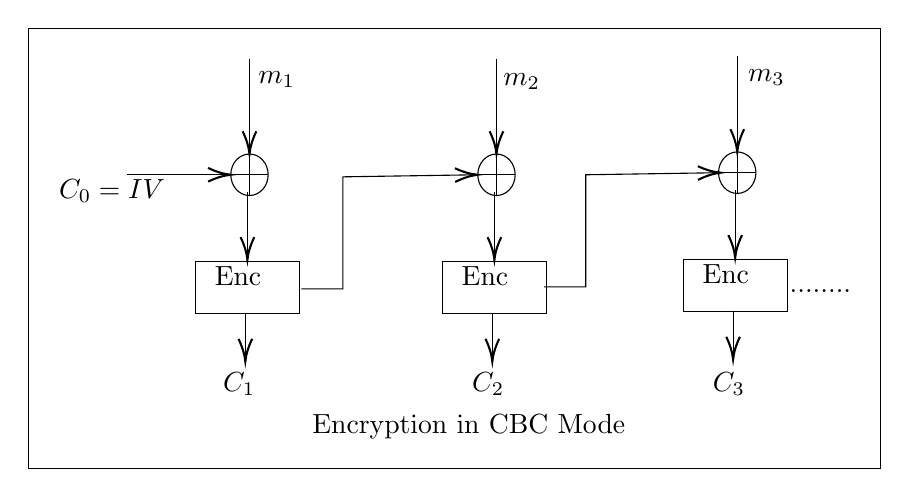
\begin{tikzpicture}[x=0.75pt,y=0.75pt,yscale=-1,xscale=1]
        \draw   (100,123) .. controls (100,117.48) and (104.03,113) .. (109,113) .. controls (113.97,113) and (118,117.48) .. (118,123) .. controls (118,128.52) and (113.97,133) .. (109,133) .. controls (104.03,133) and (100,128.52) .. (100,123) -- cycle ; \draw   (100,123) -- (118,123) ; \draw   (109,113) -- (109,133) ;
        \draw    (109,67) -- (109,111) ;
        \draw [shift={(109,113)}, rotate = 270] [color={rgb, 255:red, 0; green, 0; blue, 0 }  ][line width=0.75]    (10.93,-3.29) .. controls (6.95,-1.4) and (3.31,-0.3) .. (0,0) .. controls (3.31,0.3) and (6.95,1.4) .. (10.93,3.29)   ;
        \draw   (83,165) -- (133,165) -- (133,190) -- (83,190) -- cycle ; 
        \draw    (108,131.5) -- (108,162) ;
        \draw [shift={(108,164)}, rotate = 270] [color={rgb, 255:red, 0; green, 0; blue, 0 }  ][line width=0.75]    (10.93,-3.29) .. controls (6.95,-1.4) and (3.31,-0.3) .. (0,0) .. controls (3.31,0.3) and (6.95,1.4) .. (10.93,3.29)   ;
        \draw    (107,189.5) -- (107,211) ;
        \draw [shift={(107,213)}, rotate = 270] [color={rgb, 255:red, 0; green, 0; blue, 0 }  ][line width=0.75]    (10.93,-3.29) .. controls (6.95,-1.4) and (3.31,-0.3) .. (0,0) .. controls (3.31,0.3) and (6.95,1.4) .. (10.93,3.29)   ;
        \draw   (219,123) .. controls (219,117.48) and (223.03,113) .. (228,113) .. controls (232.97,113) and (237,117.48) .. (237,123) .. controls (237,128.52) and (232.97,133) .. (228,133) .. controls (223.03,133) and (219,128.52) .. (219,123) -- cycle ; \draw   (219,123) -- (237,123) ; \draw   (228,113) -- (228,133) ;
        \draw    (228,67) -- (228,111) ;
        \draw [shift={(228,113)}, rotate = 270] [color={rgb, 255:red, 0; green, 0; blue, 0 }  ][line width=0.75]    (10.93,-3.29) .. controls (6.95,-1.4) and (3.31,-0.3) .. (0,0) .. controls (3.31,0.3) and (6.95,1.4) .. (10.93,3.29)   ;
        \draw   (202,165) -- (252,165) -- (252,190) -- (202,190) -- cycle ;
        \draw    (227,131.5) -- (227,162) ;
        \draw [shift={(227,164)}, rotate = 270] [color={rgb, 255:red, 0; green, 0; blue, 0 }  ][line width=0.75]    (10.93,-3.29) .. controls (6.95,-1.4) and (3.31,-0.3) .. (0,0) .. controls (3.31,0.3) and (6.95,1.4) .. (10.93,3.29)   ; 
        \draw    (226,189.5) -- (226,211) ;
        \draw [shift={(226,213)}, rotate = 270] [color={rgb, 255:red, 0; green, 0; blue, 0 }  ][line width=0.75]    (10.93,-3.29) .. controls (6.95,-1.4) and (3.31,-0.3) .. (0,0) .. controls (3.31,0.3) and (6.95,1.4) .. (10.93,3.29)   ;
        \draw   (335,122) .. controls (335,116.48) and (339.03,112) .. (344,112) .. controls (348.97,112) and (353,116.48) .. (353,122) .. controls (353,127.52) and (348.97,132) .. (344,132) .. controls (339.03,132) and (335,127.52) .. (335,122) -- cycle ; \draw   (335,122) -- (353,122) ; \draw   (344,112) -- (344,132) ;
        \draw    (344,66) -- (344,110) ;
        \draw [shift={(344,112)}, rotate = 270] [color={rgb, 255:red, 0; green, 0; blue, 0 }  ][line width=0.75]    (10.93,-3.29) .. controls (6.95,-1.4) and (3.31,-0.3) .. (0,0) .. controls (3.31,0.3) and (6.95,1.4) .. (10.93,3.29)   ;
        \draw   (318,164) -- (368,164) -- (368,189) -- (318,189) -- cycle ;
        \draw    (343,130.5) -- (343,161) ;
        \draw [shift={(343,163)}, rotate = 270] [color={rgb, 255:red, 0; green, 0; blue, 0 }  ][line width=0.75]    (10.93,-3.29) .. controls (6.95,-1.4) and (3.31,-0.3) .. (0,0) .. controls (3.31,0.3) and (6.95,1.4) .. (10.93,3.29)   ;
        \draw    (342,188.5) -- (342,210) ;
        \draw [shift={(342,212)}, rotate = 270] [color={rgb, 255:red, 0; green, 0; blue, 0 }  ][line width=0.75]    (10.93,-3.29) .. controls (6.95,-1.4) and (3.31,-0.3) .. (0,0) .. controls (3.31,0.3) and (6.95,1.4) .. (10.93,3.29)   ;
        \draw    (134,178) -- (154,178) -- (154,124) -- (217,123.03) ;
        \draw [shift={(219,123)}, rotate = 179.12] [color={rgb, 255:red, 0; green, 0; blue, 0 }  ][line width=0.75]    (10.93,-3.29) .. controls (6.95,-1.4) and (3.31,-0.3) .. (0,0) .. controls (3.31,0.3) and (6.95,1.4) .. (10.93,3.29)   ;
        \draw    (251,177) -- (271,177) -- (271,123) -- (334,122.03) ;
        \draw [shift={(336,122)}, rotate = 179.12] [color={rgb, 255:red, 0; green, 0; blue, 0 }  ][line width=0.75]    (10.93,-3.29) .. controls (6.95,-1.4) and (3.31,-0.3) .. (0,0) .. controls (3.31,0.3) and (6.95,1.4) .. (10.93,3.29)   ; 
        \draw    (50,123) -- (98,123) ;
        \draw [shift={(100,123)}, rotate = 180] [color={rgb, 255:red, 0; green, 0; blue, 0 }  ][line width=0.75]    (10.93,-3.29) .. controls (6.95,-1.4) and (3.31,-0.3) .. (0,0) .. controls (3.31,0.3) and (6.95,1.4) .. (10.93,3.29)   ;
        
        \draw (91,166) node [anchor=north west][inner sep=0.75pt]   [align=left] {Enc};
        \draw (95,217) node [anchor=north west][inner sep=0.75pt]   [align=left] {$C_1$};
        \draw (210,166) node [anchor=north west][inner sep=0.75pt]   [align=left] {Enc};
        \draw (215,217) node [anchor=north west][inner sep=0.75pt]   [align=left] {$C_2$};
        \draw (326,165) node [anchor=north west][inner sep=0.75pt]   [align=left] {Enc};
        \draw (331,217) node [anchor=north west][inner sep=0.75pt]   [align=left] {$C_3$};
        \draw (368,177) node [anchor=north west][inner sep=0.75pt]   [align=left] {........};
        \draw (16,124) node [anchor=north west][inner sep=0.75pt]   [align=left] {$C_0 = IV$};
        \draw (112,72) node [anchor=north west][inner sep=0.75pt]   [align=left] {$m_1$};
        \draw (230,73) node [anchor=north west][inner sep=0.75pt]   [align=left] {$m_2$};
        \draw (348,71) node [anchor=north west][inner sep=0.75pt]   [align=left] {$m_3$};
        \draw (138,237) node [anchor=north west][inner sep=0.75pt]   [align=left] {Encryption in CBC Mode};
\node [draw, inner sep=10pt, fit=(current bounding box)] {};
    \end{tikzpicture}}
    \label{fig:your_label}
\end{figure}

\noindent
\textbf{Decryption:}
\begin{center}
    $m_i = Dec(C_i, K) \oplus C_{i-1}$ $\forall$ $i \in \{1,2...,t\}$\\
    where $C_0 = IV$\\
    $M = m_1 || m_2 || ..... || m_t$
\end{center}

\begin{figure}[H]
    \centering
    \fbox{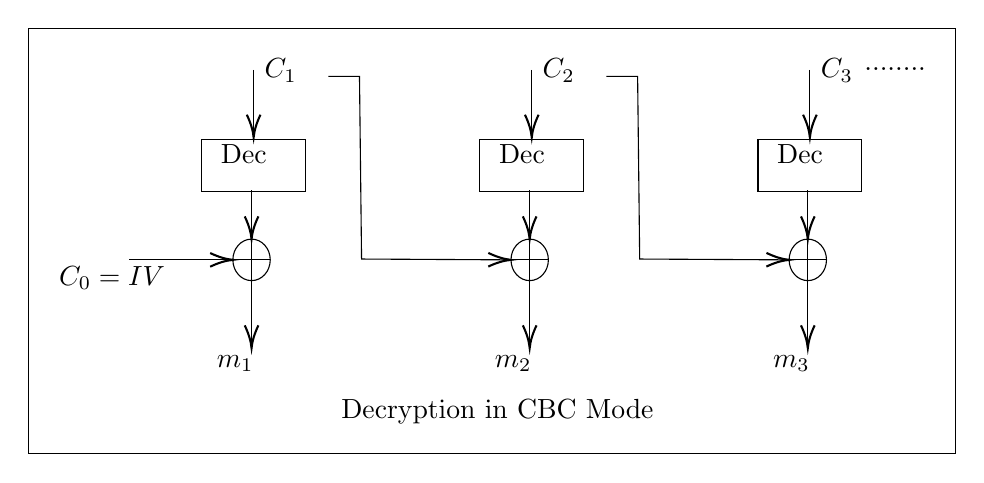
\begin{tikzpicture}[x=0.75pt,y=0.75pt,yscale=-1,xscale=1]
        \draw   (92,71) -- (142,71) -- (142,96) -- (92,96) -- cycle ; 
        \draw    (117,37.5) -- (117,68) ;
        \draw [shift={(117,70)}, rotate = 270] [color={rgb, 255:red, 0; green, 0; blue, 0 }  ][line width=0.75]    (10.93,-3.29) .. controls (6.95,-1.4) and (3.31,-0.3) .. (0,0) .. controls (3.31,0.3) and (6.95,1.4) .. (10.93,3.29)   ;
        \draw    (116,95.5) -- (116,117) ;
        \draw [shift={(116,119)}, rotate = 270] [color={rgb, 255:red, 0; green, 0; blue, 0 }  ][line width=0.75]    (10.93,-3.29) .. controls (6.95,-1.4) and (3.31,-0.3) .. (0,0) .. controls (3.31,0.3) and (6.95,1.4) .. (10.93,3.29)   ;
        \draw   (107,129) .. controls (107,123.48) and (111.03,119) .. (116,119) .. controls (120.97,119) and (125,123.48) .. (125,129) .. controls (125,134.52) and (120.97,139) .. (116,139) .. controls (111.03,139) and (107,134.52) .. (107,129) -- cycle ; \draw   (107,129) -- (125,129) ; \draw   (116,119) -- (116,139) ;
        \draw    (57,129) -- (105,129) ;
        \draw [shift={(107,129)}, rotate = 180] [color={rgb, 255:red, 0; green, 0; blue, 0 }  ][line width=0.75]    (10.93,-3.29) .. controls (6.95,-1.4) and (3.31,-0.3) .. (0,0) .. controls (3.31,0.3) and (6.95,1.4) .. (10.93,3.29)   ;
        \draw    (116,139) -- (116,169.5) ;
        \draw [shift={(116,171.5)}, rotate = 270] [color={rgb, 255:red, 0; green, 0; blue, 0 }  ][line width=0.75]    (10.93,-3.29) .. controls (6.95,-1.4) and (3.31,-0.3) .. (0,0) .. controls (3.31,0.3) and (6.95,1.4) .. (10.93,3.29)   ;
        \draw   (226,71) -- (276,71) -- (276,96) -- (226,96) -- cycle ;
        \draw    (251,37.5) -- (251,68) ;
        \draw [shift={(251,70)}, rotate = 270] [color={rgb, 255:red, 0; green, 0; blue, 0 }  ][line width=0.75]    (10.93,-3.29) .. controls (6.95,-1.4) and (3.31,-0.3) .. (0,0) .. controls (3.31,0.3) and (6.95,1.4) .. (10.93,3.29)   ;
        \draw    (250,95.5) -- (250,117) ;
        \draw [shift={(250,119)}, rotate = 270] [color={rgb, 255:red, 0; green, 0; blue, 0 }  ][line width=0.75]    (10.93,-3.29) .. controls (6.95,-1.4) and (3.31,-0.3) .. (0,0) .. controls (3.31,0.3) and (6.95,1.4) .. (10.93,3.29)   ;
        \draw   (241,129) .. controls (241,123.48) and (245.03,119) .. (250,119) .. controls (254.97,119) and (259,123.48) .. (259,129) .. controls (259,134.52) and (254.97,139) .. (250,139) .. controls (245.03,139) and (241,134.52) .. (241,129) -- cycle ; \draw   (241,129) -- (259,129) ; \draw   (250,119) -- (250,139) ;
        \draw    (250,139) -- (250,169.5) ;
        \draw [shift={(250,171.5)}, rotate = 270] [color={rgb, 255:red, 0; green, 0; blue, 0 }  ][line width=0.75]    (10.93,-3.29) .. controls (6.95,-1.4) and (3.31,-0.3) .. (0,0) .. controls (3.31,0.3) and (6.95,1.4) .. (10.93,3.29)   ;
        \draw   (360,71) -- (410,71) -- (410,96) -- (360,96) -- cycle ;
        \draw    (385,37.5) -- (385,68) ;
        \draw [shift={(385,70)}, rotate = 270] [color={rgb, 255:red, 0; green, 0; blue, 0 }  ][line width=0.75]    (10.93,-3.29) .. controls (6.95,-1.4) and (3.31,-0.3) .. (0,0) .. controls (3.31,0.3) and (6.95,1.4) .. (10.93,3.29)   ;
        \draw    (384,95.5) -- (384,117) ;
        \draw [shift={(384,119)}, rotate = 270] [color={rgb, 255:red, 0; green, 0; blue, 0 }  ][line width=0.75]    (10.93,-3.29) .. controls (6.95,-1.4) and (3.31,-0.3) .. (0,0) .. controls (3.31,0.3) and (6.95,1.4) .. (10.93,3.29)   ;
        \draw   (375,129) .. controls (375,123.48) and (379.03,119) .. (384,119) .. controls (388.97,119) and (393,123.48) .. (393,129) .. controls (393,134.52) and (388.97,139) .. (384,139) .. controls (379.03,139) and (375,134.52) .. (375,129) -- cycle ; \draw   (375,129) -- (393,129) ; \draw   (384,119) -- (384,139) ;
        \draw    (384,139) -- (384,169.5) ;
        \draw [shift={(384,171.5)}, rotate = 270] [color={rgb, 255:red, 0; green, 0; blue, 0 }  ][line width=0.75]    (10.93,-3.29) .. controls (6.95,-1.4) and (3.31,-0.3) .. (0,0) .. controls (3.31,0.3) and (6.95,1.4) .. (10.93,3.29)   ;
        \draw    (153,40.6) -- (168,40.6) -- (169,128.6) -- (239,128.99) ;
        \draw [shift={(241,129)}, rotate = 180.32] [color={rgb, 255:red, 0; green, 0; blue, 0 }  ][line width=0.75]    (10.93,-3.29) .. controls (6.95,-1.4) and (3.31,-0.3) .. (0,0) .. controls (3.31,0.3) and (6.95,1.4) .. (10.93,3.29)   ;
        \draw    (287,40.6) -- (302,40.6) -- (303,128.6) -- (373,128.99) ;
        \draw [shift={(375,129)}, rotate = 180.32] [color={rgb, 255:red, 0; green, 0; blue, 0 }  ][line width=0.75]    (10.93,-3.29) .. controls (6.95,-1.4) and (3.31,-0.3) .. (0,0) .. controls (3.31,0.3) and (6.95,1.4) .. (10.93,3.29)   ;
        
        \draw (100,72) node [anchor=north west][inner sep=0.75pt]   [align=left] {Dec};
        \draw (121,31) node [anchor=north west][inner sep=0.75pt]   [align=left] {$C_1$};
        \draw (22,131) node [anchor=north west][inner sep=0.75pt]   [align=left] {$C_0 = IV$};
        \draw (98,174) node [anchor=north west][inner sep=0.75pt]   [align=left] {$m_1$};
        \draw (234,72) node [anchor=north west][inner sep=0.75pt]   [align=left] {Dec};
        \draw (255,31) node [anchor=north west][inner sep=0.75pt]   [align=left] {$C_2$};
        \draw (232,174) node [anchor=north west][inner sep=0.75pt]   [align=left] {$m_2$};
        \draw (368,72) node [anchor=north west][inner sep=0.75pt]   [align=left] {Dec};
        \draw (389,31) node [anchor=north west][inner sep=0.75pt]   [align=left] {$C_3$};
        \draw (366,174) node [anchor=north west][inner sep=0.75pt]   [align=left] {$m_3$};
        \draw (410,35) node [anchor=north west][inner sep=0.75pt]   [align=left] {........};
        \draw (158,195) node [anchor=north west][inner sep=0.75pt]   [align=left] {Decryption in CBC Mode};
\node [draw, inner sep=10pt, fit=(current bounding box)] {};
    \end{tikzpicture}}
    \label{fig:your_label}
\end{figure}
\section{Stream Cipher}

Stream ciphers operate on the level of individual bits, encrypting data bit by bit. Let \( M = m_0m_1...m_l \), where \( m_i \in \{0, 1\} \) represents each bit of the plaintext message. The encryption process involves combining each plaintext bit \( m_i \) with a corresponding keystream bit \( k_i \) generated by the stream cipher algorithm, resulting in the ciphertext \( C \):

\[ C = M \oplus K = (m_0 \oplus k_0)(m_1 \oplus k_1)...(m_l \oplus k_l) \]\\
Where \( \oplus \) denotes the bitwise XOR operation.\\\\
\textbf{Encryption:} \( C_i = m_i \oplus K_i \)\\\\
\textbf{Decryption:} \( m_i = C_i \oplus K_i \)
\subsection{Shannon's Notion of Perfect Secrecy}


Shannon's Theorem of Perfect Secrecy stands as a fundamental principle within cryptography, rigorously defining an algorithm's perfect security as one where the ciphertext divulges no additional information about the plaintext, irrespective of an adversary's computational capabilities.\\\\
Mathematically, Shannon's theorem can be expressed as follows:\\\\
The probability of a specific plaintext message \( m_1 \) occurring, denoted as \( Pr[M = m_1] \), remains unchanged even when conditioned on a particular ciphertext \( CH_1 \), denoted as \( Pr[M = m_1|C = CH_1] \). This equality signifies that the ciphertext does not offer any extra insight into the likelihood of \( m_1 \).\\\\
For illustration, let's consider binary variables \( m \) and \( k \), where \( m \) (belonging to the set \( \{0, 1\} \)) represents the plaintext bit and \( k \) (also from the set \( \{0, 1\} \)) denotes the corresponding key bit. Assuming the probabilities of \( m \) and \( k \) being 0 are \( P \) and \( \frac{1}{2} \) respectively, and similarly for 1, we can compute the probabilities of the resulting ciphertext \( C \) as follows:

\[
\begin{align*}
Pr[C = 0] &= Pr[M = 0 \land K = 0] + Pr[M = 1 \land K = 1] \\
&= P \times \frac{1}{2} + (1 - P) \times \frac{1}{2} \\
&= \frac{1}{2} \\
Pr[C = 1] &= Pr[M = 0 \land K = 1] + Pr[M = 1 \land K = 0] \\
&= P \times \frac{1}{2} + (1 - P) \times \frac{1}{2} \\
&= \frac{1}{2}
\end{align*}
\]\\\\
This demonstrates that the resulting ciphertext \( C \) is uniformly distributed. Thus, even if the plaintext displays bias, the ciphertext remains effectively randomized, thereby preserving perfect secrecy.

\subsection{Conditions for Perfect Secrecy}

In order for a stream cipher to achieve perfect secrecy, it must fulfill the following criteria:

\begin{enumerate}
    \item \textbf{Unique Keys:} Each message must be encrypted using a different key. Reusing the same key for multiple messages can lead to potential information leakage, as patterns in the ciphertext may reveal aspects of the plaintext.
    
    \item \textbf{Key Length vs. Message Length:} The length of the key ($|K|$) should be equal to or greater than the length of the message ($|M|$). If the key length is shorter than the message length ($|K| < |M|$), padding the key with repeated bits to match the message length can introduce vulnerabilities, potentially exposing information about the plaintext.
\end{enumerate}
Adhering to these conditions ensures that the stream cipher maintains perfect secrecy, preventing any inference about the plaintext from the ciphertext, even in the presence of adversaries with significant computational resources.\\\\
For example, the Vernam cipher, also known as the \textbf{One-Time Pad (OTP)}, achieves perfect secrecy by using each bit of the key only once. However, OTP is impractical due to the challenges of securely sharing keys that are as long as the messages themselves.




%%%%%%%%%%%%%%%%%%%%%%%%%%%%%%%%%%%%%%%%%%%%
%END
 
\end{document}